\documentclass{standalone}

\usepackage{tikz} %Graphics
\usetikzlibrary{shapes.geometric, arrows}
\usepackage{amsmath}


\tikzstyle{startstop} = [ draw=none, minimum width=1.5cm, minimum height=1cm, text centered]
\tikzstyle{process} = [rectangle, rounded corners, minimum width=1.0cm, minimum height=1.0cm, text centered, draw=black, fill=blue!30]
\tikzstyle{process_score} = [circle, minimum width=1.0cm, minimum height=1.0cm, text centered, draw=black, fill=blue!30]

\tikzstyle{arrow} = [thick,->,>=stealth]
\tikzstyle{arrow_back} = [thick,<-,>=stealth]

%\usetikzlibrary{...}
\begin{document}
	\begin{tikzpicture}[node distance=6cm]
		\node (A) {
			\begin{tikzpicture}[node distance=2cm]
			\node (a1) [startstop] {$a_1$};
			\node (a2) [startstop, below of=a1] {$(...)$};
			\node (an) [startstop, below of=a2] {$a_N$};
			\node (af) [process, right of=a2] {$FC$};
			\node (end) [startstop, right of=af] {$a_o$};
			\draw [arrow] (a1) -- (af);
			\draw [arrow] (a2) -- (af);
			\draw [arrow] (an) -- (af);
			\draw [arrow] (af) -- (end);
					
			\end{tikzpicture}
	};
	\node (B) [right of=A] {
		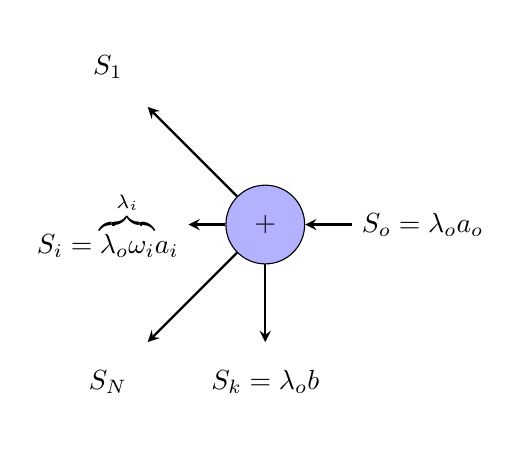
\begin{tikzpicture}[node distance=2cm]
		\node (s1) [startstop] {$S_1$};
		\node (s2) [startstop, below of=s1] {$S_i = \overset{\lambda_i}{\overbrace{\lambda_o \omega_i}} a_i$};
		\node (sn) [startstop, below of=s2] {$S_N$};
		\node (score_calc) [process_score, right of=s2] {$+$};
		\node (score_out) [startstop, right of=score_calc] {$S_o=\lambda_o a_o$};	
		\node (score_out_const)[startstop, below of=score_calc] {$S_k=\lambda_o b$};
		
		\draw [arrow_back] (s1) -- (score_calc);
		\draw [arrow_back] (s2) -- (score_calc);
		\draw [arrow_back] (sn) -- (score_calc);
		\draw [arrow_back] (score_calc) -- (score_out);	
		\draw [arrow] (score_calc) -- (score_out_const);	
		\end{tikzpicture}
	};
	\end{tikzpicture}
\end{document}

